%% This file is part of tfQMRgpu under MIT-License

\documentclass[oribibl]{llncs}

\usepackage{units}
\usepackage{psfrag} %% psfrac does not work with pdflatex
\usepackage{amssymb}
\usepackage{amsmath}
\usepackage{booktabs}
\usepackage{microtype}
\usepackage{subfigure}
\usepackage{todonotes} %% add [disable] to disable
\usepackage{transparent}
\usepackage{pgfplots}
\usepackage{gensymb} %% \degree
\usepackage{xcolor}
\usepackage{listings}

\usepackage{acronym} %% for abbreviations
%% physics related abbreviations
\acrodef{DFT}[DFT]{density functional theory}

%% computer science related abbreviations
\acrodef{CPU}[CPU]{central processing unit}
\acrodef{GPU}[GPU]{graphical processing unit}
\acrodef{HPC}[HPC]{high performance computing}
\acrodef{OMP}[OpenMP]{OpenMP}
\acrodef{MPI}[MPI]{message passing interface}


\setlength{\tabcolsep}{6pt}

\newcommand{\um}[1]{_{\mathrm{#1}}}
\newcommand{\ttt}[1]{\texttt{#1}}
\newcommand{\lmax}{\ell_{\mathrm{max}}}
\newcommand{\ellm}{L}
\newcommand{\nrn}{n_{\mathrm{r}}}
\newcommand{\ket}[1]{\left| #1 \right\rangle}
\newcommand{\bra}[1]{\left\langle #1 \right|}
\newcommand{\braket}[2]{\left\langle \left. #1 \right| #2 \right\rangle}
\newcommand{\braketop}[3]{\left\langle \left. #1 \right| #2 \left| #3 \right. \right\rangle}

\newcommand{\fullcodename}{transpose-free Quasi Minimal Residual method on GPUs}
\newcommand{\codename}{tfQMRgpu}

\begin{document}
\pagestyle{plain}

\title       {User Manual for \codename{}}
\titlerunning{\codename{} User Manual}

\author{%
  Paul F.~Baumeister\inst{1} % \and %
}

\institute{%
  J\"{u}lich Supercomputing Centre, Forschungszentrum J\"{u}lich, 52425 J\"{u}lich, Germany
%   \and Institute for Advanced Simulation, Forschungszentrum J\"{u}lich, 52425 J\"{u}lich, Germany
}

\maketitle

\begin{figure*}
	\centering
	\includegraphics[width=3cm]{logo/tf_QMR.png} %%
\end{figure*}

% ==============================================================================
\begin{abstract}
This is a user manual for the linear system solver \codename{} on GPUs.
The \fullcodename{} 
\end{abstract}
% ==============================================================================

\section*{How to read this document?}
\todo[inline]{Write}

% ==============================================================================
\section{Introduction} \label{sec:intro}
% ==============================================================================
%
In many situations we need to solve inverse problems like finding $X$ in
\begin{equation}
	A \times X = B
\end{equation}
where $B$ and $X$ are vectors and $A$ is a linear operator which could be represented
as a square matrix. \codename{} is an implementation for linear system solves,
where $X$ and $B$ are collections of column vectors treated as block-sparse matrices.

\subsection{Development background} \label{sec:backstory}
%
In the framework of electronic structure calculations with \ac{DFT},
the core problem can either be solved by an eigenvalue solver finding eigenfunction (wave functions)
or by a linear solver finding the Green function.
\codename{} has been originally developed for \emph{KKRnano}, a linear-scaling Green function \ac{DFT} application.
From this, the matrix structures are block-sparse due to the nature of a short-ranged tight-binding interaction of orbitals on neighbouring atoms and due to the truncation of the Green function.
KKRnano achieves linear scaling by truncating the Green function at a certain radius.
This leads to a special solver in which $A, X$ and $B$ are block-sparse matrices.
Since such a special solver was not found in the literature \codename{} was developed to fill this gap.
In order to leverage modern \ac{HPC} systems, the library has been written in CUDA
to harvest ther perforance of one NVIDIA \ac{GPU}.

\subsection{Library Features} \label{sec:features}
%
\codename{} can be built without \ac{GPU}-support, however,
the performance is inferior to that of libraries tuned for a \ac{CPU}.

\noindent
\codename{} is developed in CUDA \ttt{C++}.
For the standard case that the operator $A$ is also a block-sparse matrix
it comes with a \ttt{C} and a Fortran90 interface.

\subsection{Limitations}
%
The matrices $X$ and $B$ may both be block-sparse with the same block dimensions, but
wherever $B$ has a non-zero element, $X$ must have one, too.
This means $B$ may contain less elements than $X$.
Due to internal number formats the number of block rows 
and the number of non-zero elements in all blocks-sparse operators 
is limited to $2^{31}$-$1 = 2,147,483,647$ 
and the number of block columns in $X$ and $B$ 
is limited to $2^{16} = 65,536$.
Internally, \codename{} achieves \ac{GPU} performance by loop-unrolling.
This technique only works if the block dimensions are known at compile time.
Users must ensure that their required combination of block dimensions are included in the list
\ttt{tfQMRgpu/include/allowed\_block\_sizes.h}.

\todo[inline]{write a test case for limit numbers}

\noindent
\codename{} uses complex numbers in single and double precision. A purely real version is so far not available.

\section{How to get started} \label{sec:how-to-get-started}
%
\subsection{Getting the Code} \label{sec:getting-the-code}
\codename{} is public domain software under the MIT license
and can be cloned at \ttt{github.com/real-space/tfQMRgpu}.
Please follow the instruction in \ttt{README.md} to install the code

\subsection{Comments for JSC Systems}
On JUSUF please run
\begin{verbatim}
	module --force purge
	module load Stages/2020 GCC/9.3.0 CUDA/11.3 CMake
\end{verbatim}
before you run \ttt{cmake}.

\subsection{Block sparse matrices} \label{sec:bsr}
%
The interface requires a BSR (block-compress sparse row) format for matrices.
This is equivalent to the CSR (compressed sparse row) format for sparse matrices with scalar elements.
A matrix descriptor has the following fields
\begin{verbatim}
int       nRows
int32_t   rowPtr[nRows + 1] 
int       nnzb 
int32_t   colInd[nnzb]
matrix_t  mat[nnzb]
\end{verbatim}
where \ttt{nRows} gives the number of block rows and \ttt{nnzb} the total number of non-zero elements.
In this particular case a non-zero element is a block matrix which differs from an all-zero block matrix.
4-byte signed integers \ttt{int32\_t} are used for list arrays as they are equivalent to Fortran \ttt{integer(kind=4)}.
\ttt{rowPtr} gives the start of each row, i.e.~typically \ttt{rowPtr[0]} is $0$ and \ttt{rowPtr[nRows] == nnzb}.
There are as many column indices in \ttt{colInd} as there are non-zero matrix blocks.
In \ttt{C} the sparse matrix is traversed like this
\lstset{language=C}
\begin{lstlisting}
for (int irow = 0; irow < nRows; ++irow) {
  	for (int32_t inzb = rowPtr[irow]; inzb < rowPtr[irow + 1]; ++inzb) {
		int32_t  jcol = colInd[inzb];
		matrix_t A_ij = mat[inzb];
  	}
}
\end{lstlisting}
As visible from this code snippet, \ttt{rowPtr[row + 1]} is used as end of the row.
\\
\noindent
In Fortran, all indices are shifted by $1$:
\lstset{language=Fortran}
\begin{lstlisting}
do irow = 1, nRows
	do inzb = rowPtr(irow), rowPtr(irow + 1) - 1
		jcol = colInd(inzb)
		A_ij(:,:) = mat(:,:,inzb)
	end do
end do
\end{lstlisting}


\begin{figure}
	\centering
	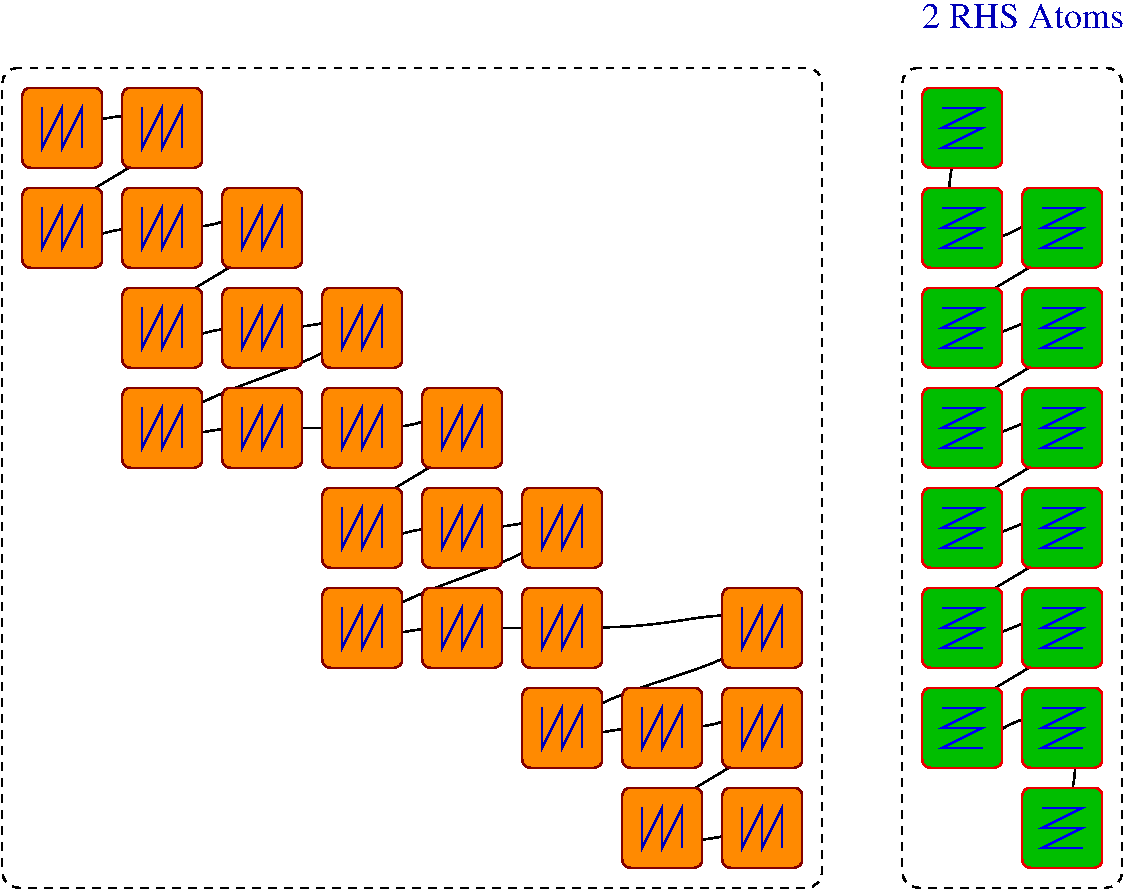
\includegraphics[width=\textwidth]{pics/rowBSR.png} %%
	\caption{Data layout internal to tfQMRgpu for the case of a block-sparse operator $A$. 
	Block elements of $A$ are stored transposed for a better usage of cache lines.
	The block ordering follows the compressed sparse row format (CSR).}
\end{figure}

\subsection{Interfacing}
%
\codename{} has been designed to allow an efficient usage of resources, in particular
memory capacity, memory accesses and setup overheads.
Often, the first question to be answered is if the user's project can benefit from \codename{}.
Therefore, \codename{} offers a comfort function \ttt{tfqmrgpu\_bsrsv\_z} in \ttt{tfQMRgpu/include/tfqmrgpu.h}:
\lstset{language=C}
\begin{lstlisting}
int tfqmrgpu_bsrsv_z(int nRows, int ldA, int ldB,
    int32_t const* rowPtrA, int nnzbA, int32_t const* colIndA,
    double const* Amat, char transA,
    int32_t const* rowPtrX, int nnzbX, int32_t const* colIndX,
    double      * Xmat, char transX,
    int32_t const* rowPtrB, int nnzbB, int32_t const* colIndB,
    double const* Bmat, char transB,
	int32_t *iterations, float *residual, int echo);
\end{lstlisting}
with the following arguments
\begin{itemize}
	\item \ttt{nRows} is the number of block rows in $A$, $X$, and $B$, and the number of block columns in $A$.
	\item \ttt{ldA} is the block dimension of blocks of $A$, i.e.~$A_{ij} \in \mathbb{C}^{\ttt{ldA}\times\ttt{ldA}}$
	\item \ttt{ldB} is the leading dimension of blocks in $X$ and $B$, e.g.~$X_{jk} \in \mathbb{C}^{\ttt{ldA}\times\ttt{ldB}}$
	\item \ttt{rowPtr}, \ttt{nnzb}, \ttt{colInd}, \ttt{mat} for $A$, $X$ and $B$ as described in Sec.~\ref{sec:bsr}.
	\item \ttt{trans} for $A$, $X$ and $B$ determines the block transpositions.
	\item \ttt{iterations} controls the maximum number of iterations and returns the number of iterations performed.
	\item \ttt{residual} controls the convergence threshold and returns the error residual reached.
	\item \ttt{echo} is a verbosity controller between \ttt{0} (no output) and \ttt{9} (debug level).
\end{itemize}

\noindent
Block transpositions must be one of \{\ttt{'n'}: non-transposed, \ttt{'t'}: transposed, \ttt{'*'}: complex-conjugated, \ttt{'h'}: Hermitian-adjoint\}. For consistency with the BLAS level 3 routine \ttt{ZGEMM} also \ttt{'c'} instead of \ttt{'h'} can be used for the combination of complex-conjugated and transposed.
Mind that \ttt{Xmat} has no \ttt{const} specifyer since this array returns the result.
\codename{} does not support the transposition of the BSR descriptors.

\subsubsection{Fortran}
Similar to this \ttt{C} interface, \ttt{tfqmrgpu\_bsrsv\_rectangular} is offered in the Fortran90 module \ttt{tfqmrgpu} from \ttt{tfQMRgpu/include/tfqmrgpu\_Fortran\_module.F90}. The only differences are indices shifted by $1$ and a final argument \ttt{ierr} which controls debug checks if nonzero and returns the error code (inspired by MPI routines).

\section{User-defined linear operators}
%
The action of the linear operator $A$ in \codename{} is a \ttt{C++} template class.
This means that \ttt{C++} users can exploit the infrastructure offered by \codename{} and exchange
the block-sparse operator $A$ against a user-defined action. The action is defined as
\begin{equation}
	Y := A \times X
\end{equation}
where $Y$ uses the same sparse descriptor as $X$.
Please refer to the class \ttt{blocksparse\_action\_t} in \ttt{include/tfqmrgpu\_blocksparse.hxx}
to see how the standard operator is constructed.
Mind that the action's \ttt{multiply} function needs to accept three \ac{GPU} memory pointers, i.e.˜˜~memory allocated with either \ttt{cudaMalloc} or \ttt{cudaMallocManaged}.

% ==============================================================================
\bibliographystyle{plain} 
\bibliography{literature}
% ==============================================================================

\end{document}
